The trade-off between determinism and nondeterminism is a central theme in automata theory. For automata over infinite words, nondeterministic B\"uchi automata are more expressive and succinct than their deterministic counterpart and, in fact, are as expressive as deterministic parity automata and exponentially more succinct~\cite{McN66,Saf88}. Even though nondeterminism seems attractive because of these favourable qualities, it presents difficulties in contexts like reactive synthesis or runtime verification when the specifications are expressed as automata. The
fundamental challenge here arises because any algorithm operating with nondeterministic automata needs to account for any possible future inputs.

Some attempts have evolved that involve modifying algorithms to avoid or minimise the blow-up using determinisation procedures~\cite{KPV06,KV05,EKS16}, while other attempts instead focus on building classes of automata that bridge this gap between determinism and nondeterminism to obtain the best of both worlds, while avoiding exponential determinisation procedures. 
The latter of the attempts include defining several classes of automata like history-deterministic (HD) automata~\cite{HP06}, good-for-MDP automata~\cite{HPSS0W20}, semantically deterministic automata~\cite{KS15,AK20}, and explorable automata~\cite{HK23} to name a few. 

The notion of history-determinism, which has inspired this work, has gained significant attention in recent years, since it allows for on-the-fly resolution of nondeterminism, which make them relevant for the problems of model-checking, and reactive synthesis~\cite[Page 22]{BL23}. 

Notably, history-deterministic automata are exponentially more succinct than deterministic automata \cite[Theorem 1]{KS15}, and history-deterministic coB\"uchi automata give rise to a canonical representation of coB\"uchi as well as $\omega$-regular languages~\cite{AK22,ES22}. History-deterministic automata are nondeterministic automata whose nondeterminism can be resolved on-the-fly and only based on the prefix of a word read so far. 
More precisely, history-determinism of an automaton can be characterised by the following history-determinism game (HD game) on that automaton. The HD game is played between two players, Eve and Adam, on an arena of the automaton where Eve initially has a token at the start state. In each round of a play, Adam picks a letter, and Eve moves her token along a transition on the letter picked by Adam, thereby constructing a run on the word that Adam has picked so far. The game proceeds for an infinite duration, where Adam constructs an infinite word, and Eve produces a run on this word. Eve wins if she has a strategy that ensures that she constructs an accepting run whenever the infinite word given by Adam is in the language of the automaton. HD automata are defined as  automata in which Eve wins the HD game. For a sanity check, consider deterministic automata, where Eve trivially wins the HD game by choosing the unique deterministic transition on each letter to produce an accepting run whenever the word is in the language. 

Such a definition of resolving nondeterministic choices as in HD automata is useful to represent winning conditions in games against an adversary, thus also being dubbed good-for-games automata at the time of its introduction~\cite[Theorem 3.1]{HP06}. This property also makes history-deterministic automata relevant for the problems of reactive synthesis and model checking~\cite[Section 7]{BL23}.
%Therefore, history-deterministic automata are valuable for reactive synthesis in an $\omega$-regular setting and further connections to simulation~\cite{BHLP24} strengthen their importance. 

Although history determinism is a useful concept, it is based on a highly adversarial setting for the player who resolves the nondeterminism. 
For example, consider the infinite word reachability automaton in~\cref{fig:ReachSRbutnotHD}, which accepts all infinite words over $\{a,b\}$.
In order to resolve the nondeterministic decision in state $q_0$ and eventually reach state $q_f$, the letter that is to be read in the next step must be guessed.  
If successive letters are chosen adversarially and based on the current state of the automaton, no resolver can successfully resolve the nondeterminism on all words, and therefore this automaton is not HD. 
\begin{figure}[ht]
    \centering
    \begin{subfigure}[t]{0.4\textwidth}
    \centering
    \begin{tikzpicture}
        \tikzset{every state/.style = {inner sep=-3pt,minimum size =20}}

    \node[state] (q0) at (0,0) {$q_0$};
    \node[state] (qa) at (1.2,1.5) {$q_a$};
    \node[state] (qb) at (1.2,-1.5) {$q_b$};
    \node[state] (qf) at (2.4,0) {$q_f$};
    \path[-stealth]
    (-0.75,0) edge (q0)

  
    (q0) edge [bend left = 30] node [above, yshift = 1] {$a,b$} (qa)
    (q0) edge [bend right = 30] node [below, yshift = -2] {$a,b$} (qb)
    (qa) edge node [below] {$b$} (q0) 
    (qb) edge node [above] {$a$} (q0)
    (qa) edge node [above] {$a$} (qf)
    (qb) edge node [below] {$b$} (qf)
    (qf) edge [double, loop above] node [above] {$a,b$} (qf)
    ;
    \end{tikzpicture}
    \caption{A reachability automaton that is not history deterministic.}
    \label{fig:ReachSRbutnotHD}
    \end{subfigure}~~~
    \begin{subfigure}[t]{0.4\textwidth}
    \centering
        \begin{tikzpicture}
        \tikzset{every state/.style = {inner sep=-3pt,minimum size =20}}

    \node[state] (q0) at (0,0) {$s$};
    \node[state] (qa) at (2,1.5) {$s^\circ$};
    \node[state] (qb) at (2,-1.5) {$s_\circ$};
    \path[-stealth]
    (-0.75,0) edge (q0)
    (q0) edge [bend left = 10] (qa)
    (q0) edge [bend right = 10] (qb)
    (qa) edge[red, dashed,bend left =10] (q0) 
    (qb) edge[red, dashed,bend right =10]  (q0)
    (qa) edge[bend right =10]  (qb)
    (qb) edge[bend right =10]  (qa)
    (q0) edge[loop above] (q0)
    (qa) edge[loop right] (qa)
    (qb) edge[loop right] (qb)
    ;
    \node (l1) at (0,1) {$\swapletter$};
    \node (l2) at (2.4,0) {$\swapletter$};
    \node (l3) at (1.6,0) {$\swapletter$};

%    \node (l4) at (0,1) {$\sameletter$};
    \node (l5) at (3.2,1.5) {$\sameletter\!,\!\!\upletter$};
    \node (l6) at (3.2,-1.5) {$\sameletter\!,\!\!\downletter$};  
    
    \node (l4) at (0.7,1.1) {$\sameletter\!,\!\!\upletter$};
    \node (l7) at (0.7,-1.1) {$\sameletter\!,\!\!\downletter$};   
    
    \node (l8) at (1.1,0.4) {$\downletter$};
    \node (l9) at (1.1,-0.4) {$\upletter$};   
    \end{tikzpicture}
    \caption{A HD coB\"uchi automaton where nondeterminism can be resolved randomly}
    \label{fig:coBuchiEx}
    \end{subfigure}
    \caption{Examples of resolving nondeterminism with randomness}
\end{figure}
However, in a more lenient setting where the adversary pre-commits to an infinite word, a resolver that resolves the nondeterminism by choosing uniformly at random one of the two transitions from $q_0$ would produce an accepting run almost surely, that is, with probability 1. 
%In this less adversarial settings of the adversary, history determinism is a stronger notion than required. 

%Even in the adversarial setting, randomness is a useful tool to resolve the nondeterminism. 
Allowing for stochastic resolvers simplifies the memory structure of the resolvers even for HD automata. 
Consider the coB\"uchi automaton in \cref{fig:coBuchiEx} inspired from the work of Kuperberg and Skrzypczak~\cite[Theorem~1]{KS15}. Accepting runs in a coB\"uchi automaton must visit rejecting (dashed) transitions only finitely often. The language of the auomaton is over the alphabet $\{\!\!\swapletter\!,\!\sameletter\!,\!\upletter\!,\!\downletter\!\!\}$ and therefore, each infinite word naturally constructs an infinite graph over  $\Nb\times \{1,2\}$. 
We demonstrate with the finite word $\!\!\swapletter\!\!\!\sameletter\!\!\!\sameletter\!\!\!\swapletter\!\!$ that represents a graph with two distinct finite paths of length 4, if the right-most dots of a letter are identified with the left-most dots of the next letter in the word.  
The infinite word 
$(\!\!\swapletter\!\!\!\sameletter\!\!\!\sameletter\!\!\!\swapletter\!\!)^\omega$ represents a graph with two infinite paths. %, and so does any word in the language 
%$\tpl{\!\!\swapletter\!\!\!+\!\!\!\sameletter\!\!}^\omega$. 
However, the word
$(\!\!\swapletter\!\!\!\upletter\!\!\!\sameletter\!\!)^\omega$ does not have any infinite path, as the letter $\!\!\upletter\!\!$ breaks each path infinitely often. %, but the word $\tpl{\!\!\swapletter\!\!\!\upletter\!\!\!\sameletter\!\!\!\swapletter\!\!}^\omega$ has one infinite path despite the infinite occurrence of the same letter. 
It can be verified that the nondeterministic coB\"uchi automaton in \cref{fig:coBuchiEx} accepts an infinite word if and only if the corresponding graph has at least one infinite path.  
Indeed, the two nondeterministic choices correspond to verifying if the path starting from the bottom vertex is infinite or the top vertex is infinite, respectively. A correct guess ensures that rejecting transitions never occur in the run and a wrong guess brings the run back to the start vertex from which a guess needs to be made again. 

%There is a strategy to resolve the nondeterminism against any adversarially constructed input sequence of letters in this automaton, and therefore it is HD. 
This automaton is history-deterministic. Consider the resolver that chooses the transition from state $s$ that follows the longest unbroken path so far to verify that it extends to an infinite path. If there is an infinite path then eventually it would be the longest unbroken path, and such a resolver would correctly resolve the nondeterminism to produce an accepting run. Note that any resolver that selects a transition from $s$ uniformly at random also constructs an accepting run on any infinite word in the language with probability~$1$, even if letters are chosen adversarially and based on the current state. This is the case because the run of the resolver would, with probability~$1$, eventually coincide with one of the longest unbroken paths. %This randomised resolver ensures that the constructed run is accepting with probability~$1$, trading memory for randomness. 
% For checking SR on the other hand, the problem of checking if a given resolver is an almost-sure resolver is undecidable in the case of B\"uchi or coB\"uchi automata. This makes our result that we can convert any SR coB\"uchi automaton to a MA coB\"uchi automaton in \cref{sec:succandcomp}, all the more surprising.
% in this resolver. %, irrespective of any adversary's choices. 
% This strategy requires memory, which continues the longest path seen so far in the past. However, equivalently, another strategy could be to resolve the nondeterminsm, and even if the input letters are chosen adversarially, if the word is in the language, almost surely, the run produced would be an accepting run. 

%These examples therefore motivates the settings we consider. 

%A parity automaton is a finite state automaton where each transition is equipped with a natural number, called priority. A run of the automaton is accepting if the largest priority occurring infinitely often is even. 
Motivated by these examples, we introduce classes of automata inspired by history determinism, extending them in two ways. First, we consider resolvers that use not only memory but also stochasticity, and second, we also study settings where the letter-giving adversary commits to a word in advance.%\theju{weaker?}   
% This paper introduces and studies categories of nondeterministic parity automata  within two different adversarial frameworks, where the nondeterminism in automata can be resolved on-the-fly using both memory and randomness.

\paragraph*{New classes of automata} Intuitively, stochastic resolvers propose an outgoing transition using both memory and randomness.
We study classes of automata for which there is an \emph{almost-sure} resolver, a policy for resolving the nondeterminism (which can use memory or randomness) such that for all words in the language, the run produced is almost-surely accepting, that is, with probability~1.% under two different settings.

We consider the existence of almost-sure resolvers in the following two settings for the letter-giving adversary.  The first setting, called \emph{adversarial resolvability}, is where the input words to the automaton are from an adversary that generates the input letter-by-letter based on the resolution of the nondeterminism in the past. This definition is reminiscent to the definition of resolvers in history determinism, where now we allow for stochasticity. Indeed, the resolvers here represent the strategy of Eve in the HD game defined for history determinism, where we allow for a larger class of resolvers which allow for randomness. 
The second, and novel setting, called \emph{stochastic resolvability}, is where the adversary commits to an entire input-word, but only reveals the input letter-by-letter to their opponent who is resolving the nondeterminism. 
%Similar to the letter game, we can define an SR game, where such a letter-giving adversary can also be equivalently viewed as an opponent that does not have access to any of the internal coin-tosses of the almost-sure resolver of the non-determinism. This can also be equivalently formulated by a partial observation game similar to the letter game defined. The turn of the games proceed similar to the letter game, but Adam is \emph{blind} to the moves of Eve in the game and has no view of the token of Eve.

 We call the class of automata that have an almost-sure resolver in the adversarial resolvability setting as \emph{adversarially resolvable automata}, and that have an almost-sure resolver in the stochastic resolvability setting as \emph{stochastically resolvable automata}, or SR automata, for short.
We further study the classes of automata where ``weaker'' resolvers are used. If the resolvers of nondeterminism are restricted to policies where no memory and only stochasticity is used, then the resolving strategy is just a probability distribution among the outgoing transition for each state. We call such classes of resolvers \emph{memoryless resolvers}, and the class of automata that are adversarially resolvable using memoryless almost-sure resolvers as \emph{memoryless-adversarially resolvable}, or MA for short. Likewise, we call the class of automata that are stochastically resolvable using memoryless almost-sure resolvers \emph{memoryless-stochastically resolvable}, or MR for short. The class of adversarially resolvable automata, without any restrictions on resolvers, are equivalent to HD automata due to determinacy of $\omega$-regular games.

\paragraph*{Our results}
We introduce and then make comparisons between the three newly introduced classes of automata and also with existing notions such as HD automata and semantically deterministic (SD) automata (automata where every nondeterministic transition leads to language equivalent states)~\cite{AK23}, and we study the questions of succinctness, expressivity, and computational complexity of the class-membership problem for these automata classes. 

%while making distinctions between these classes by providing separating examples. 

% In all generality, adversarially resolvable automata are equivalent to history-deterministic automata. But when restricted to memoryless resolvers, MA automata forms a smaller subclass of HD automata for B\"uchi, coB\"uchi, and parity automata. 
In \cref{sec:succandcomp}, we compare our novel automata classes with each other and also with history-deterministic and semantically deterministic automata. We show separating examples or prove the equivalences between the classes (\cref{theorem:comp}). A landscape of these automata can be found in \cref{fig:venndiagrammmmmm}.
\begin{figure}[h]
    \centering
    \begin{minipage}[b]{0.4\linewidth}
            \begin{subfigure}[b]{\linewidth}
        \centering
        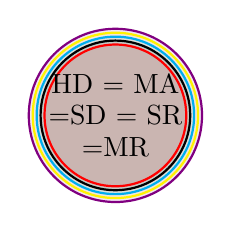
\begin{tikzpicture}
            \draw[thick,violet] (0,0) circle (1.1cm);
            \fill[violet, opacity=0.1] (0,0) circle (1.1cm);
            
            \draw[thick,yellow] (0,0) circle (1.05cm);
            \fill[yellow, opacity=0.1] (0,0) circle (1.05cm);
            
            \draw[thick,cyan] (0,0) circle (1cm);
            \fill[cyan, opacity=0.1] (0,0) circle (1cm); 

            \fill[black, opacity=0.1] (0,0) circle (0.95cm);;
            \draw[thick,black] (0,0) circle (0.95cm);
            
            \draw[thick,red] (0,0) circle (0.9cm);
            \fill[red, opacity=0.1] (0,0) circle (0.9cm);

            \node at (0,0.4) {HD = MA};
            \node at (0,0) {=SD = SR};
            \node at (0,-0.4) {=MR};
        \end{tikzpicture}
    \caption{Safety}
    \end{subfigure}%
    \vfill
    \begin{subfigure}[b]{\linewidth}
        \centering
        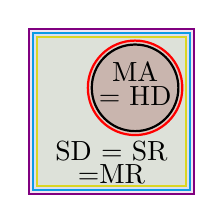
\begin{tikzpicture}
            \draw[thick,cyan] (-1,1) rectangle (1,-1);
            \draw[thick,yellow] (-0.95,0.95) rectangle (0.95,-0.95); % Object 4
            \fill[violet, opacity=0.1] (-1.05,1.05) rectangle (1.05,-1.05);
            \fill[cyan, opacity=0.1] (-1,1) rectangle (1,-1); 
            \fill[yellow, opacity=0.1] (-0.95,0.95) rectangle (0.95,-0.95);
            \draw[thick,violet] (-1.05,1.05) rectangle (1.05,-1.05);

            
            \draw[thick,red] (0.3,0.3) circle (0.6cm);
            \fill[red, opacity=0.1] (0.3,0.3) circle (0.6cm);
            \draw[thick,black] (0.3,0.3) circle (0.55cm);
            \fill[black, opacity=0.1] (0.3,0.3) circle (0.55cm);
            \node at (0,-0.5) {SD = SR};
            \node at (0,-0.8) {=MR};
            \node at (0.3,0.5) {MA};
            \node at (0.3,0.2) {= HD};
        \end{tikzpicture}
    \caption{Reachability, Weak}
    \end{subfigure}%
    \end{minipage}
    \hfill
    \begin{minipage}[b]{0.5\linewidth}
        \begin{subfigure}[b]{\linewidth}
        \centering
        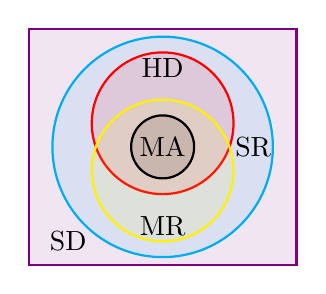
\begin{tikzpicture}
            \draw[thick,violet] (-1.7,1.5) rectangle (1.7,-1.5);
            \fill[violet, opacity=0.1] (-1.7,1.5) rectangle (1.7,-1.5);% Object 1
            \draw[thick,cyan] (0,0) circle (1.4cm);
            \fill[cyan, opacity=0.1] (0,0) circle (1.4cm); % Object 2
            \draw[thick,red] (0,0.3) circle (0.9cm); % Object 3
            \fill[red, opacity=0.1] (0,0.3) circle (0.9cm);
            \draw[thick,yellow] (0,-0.3) circle (0.9cm); % Object 4
            \fill[yellow, opacity=0.1] (0,-0.3) circle (0.9cm);
            \fill[black,opacity=0.1] (0,0) circle (0.4cm);
            \draw[black,thick] (0,0) circle (0.4cm); % Object 5
            \node at (-1.2,-1.2) {SD};
            \node at (1.15,0) {SR};
            \node at (0,1) {HD};
            \node at (0,-1) {MR};
            \node at (0,0) {MA};
        \end{tikzpicture}    \caption{B\"uchi, co-B\"uchi, Parity}
    \end{subfigure}
    \caption{The landscape of automata that admit different resolvers}\label{fig:venndiagrammmmmm}
    \end{minipage}
\end{figure}
In the same section, we show \emph{exponential succinctness of SR coB\"uchi to deterministic B\"uchi automata and SR B\"uchi automata to HD B\"uchi automata (\cref{theorem:succ})} %automaton are exponentially more succinct than HD B\"uchi automata} (\cref{theorem:succ}). 
For coB\"uchi automata on the other hand, we show a surprising result that \emph{any SR coB\"uchi automaton can be converted into an MA automaton with the same number of states} (\cref{theorem:coBuchiHDisSR}). This result, therefore, shows that SR coB\"uchi automata are no more succinct than HD coB\"uchi~automata. %, but exponentially than deterministic coBu\"uchi automata (\cref{theorem:succ}) %But we show that B\"uchi SR automata are exponentially succinct than even HD automata.

In \cref{sec:pih}, we turn our attention to the problem of expressivity.  History-deterministic (and therefore also MA) parity automata that use priorities from $\{i,i+1,\dots,j\}$ are as expressive as their deterministic counterparts~\cite{BKS17}. We show that SR and MR automata are similar to HD automata in this regard by showing that \emph{the parity index hierarchy for SR automata is strict} (\cref{theorem:pih}). 

Finally, in \cref{sec:complexity}, we tackle the problems of deciding if an automata is MA and SR. The exact complexity of the problem of deciding if an automaton is HD is an open problem since the introduction of the class in 2006~\cite{HP06}, with recent improvements giving the problem a $\NP$ lower bound~\cite{Pra24a} and a $\PSPACE$ upper bound~\cite[2-Token Theorem]{LP25, Pra25}.
We show that the situation for MA automata is better as we show that \emph{checking if an automaton is MA is $\NP$-complete} (\cref{theorem:manpcomplete}). The upper bound relies on showing that a slight modification of the 2-token game~\cite{BK18,LP25}, a game used to characterise history deterministic automata, also characterises MA automata. With such a characterisation, we show that to check if an automata is MA, one first needs to guess a strategy in the modified two-token game. Checking correctness of this strategy reduces to solving a Markov decision process (MDP) with Muller objective, where objective can be represented succinctly using a Zielonka DAG. We show that this can be computed in polynomial time (\cref{thm:ZlkDAGMDP}). This result on MDPs was only previously known for less succinct representations of Muller objectives~\cite{Cha07}.  We also consider problems related to checking whether an automaton is in the class MR and SR. We summarise the results of the decision procedures discussed in~\cref{table:TomwantsTables}.

\iffalse

\begin{table*}[t]
\centering
\begin{tabular}{| l || c | c | c | c | c | c | }
\hline
 & Safety & Reachability/Weak & Buchi & coB\"uchi & Parity\\
\hline\hline
Checking MA (\cref{theorem:manpcomplete}) & $\P$ & $\P$   & $\NP$ & $\NP$  & $\NP$-complete \\
\hline
Checking HD & $\P$~\cite{KS15,BL23quantitative} & $\P$~\cite{KS15,BL23quantitative}    & $\P$~\cite{KS15} & $\P$~\cite{BK18}  & \parbox{2.5cm}{$\PSPACE$~\cite{LP25}, $\NP$-hard~\cite{Pra24a}} \\
\hline
Checking SR/ MR (\cref{theorem:complexity}) & $\P$ & $\PSPACE$-comp  & Open & Open & Open\\ 			\hline
Resolver checking for SR/MR (\cref{theorem:complexity}) & $\P$ & $\PSPACE$-comp  & undec. & undec. & undec.\\
  \hline 
\end{tabular}
\caption{Complexity of checking membership of an automaton in a class.}
\label{table:TomwantsTables}
\end{table*}

\fi 

\begin{table*}[t]
\centering
\begin{tabular}{| l || c | c | c | c | c | c | }
\hline
 & Safety & Reachability/Weak & Buchi & coB\"uchi & Parity\\
\hline\hline
\parbox{3cm}{Checking MA (\cref{theorem:manpcomplete})} & $\P$ & $\P$   & $\NP$ & $\NP$  & $\NP$-complete \\
\hline
Checking HD & $\P$~\cite{KS15,BL23quantitative} & $\P$~\cite{KS15,BL23quantitative}    & $\P$~\cite{KS15} & $\P$~\cite{BK18}  & \parbox{2.5cm}{$\PSPACE$~\cite{LP25}, $\NP$-hard~\cite{Pra24a}} \\
\hline
\parbox{3cm}{Checking SR/ MR (\cref{theorem:complexity})} & $\P$ & $\PSPACE$-comp  & Open & Open & Open\\ 			\hline
\parbox{3cm}{Resolver checking for SR/MR (\cref{theorem:complexity})} & $\P$ & $\PSPACE$-comp  & undec. & undec. & undec.\\
  \hline 
\end{tabular}
\caption{Complexity of checking membership of an automaton in a class.}
\label{table:TomwantsTables}
\end{table*}

